Until Edwin Hubble's measurement of the distances to M31 and M33 using Cepheid variable stars in the early twentieth century (\citealt{Hubble_1925}), many astronomers believed that the Milky Way encompassed all matter in the Universe. Observational data of the time meant that all extragalactic sources, appearing as small, hazy patches of light in the sky, were indistinguishable from clusters of stars, gas and dust that are part of our own Galaxy. Objects that were not immediately identifiable as stars were given the name \textit{nebulae} (Latin for 'clouds') which included Galactic sources as well as hitherto unknown extragalactic sources such as the \textit{Andromeda Nebula}. The consequence of this confusion is still evident in astronomy today in the naming convention used for certain catalogues, such as the Messier Catalogue, which consists of star clusters, nebulae and supernova remnants within the Galaxy as well as other galaxies, including \textit{Andromeda} (M31).

Since this initial discovery, the number of catalogued galaxies in the observable Universe has been ever increasing. Thanks to the finite speed of light, the history of star formation in the Universe can be observed directly from the light of distant galaxies as we look back time. Deep observations allow us to explore the evolution of galaxies from the early Universe to the galaxies we observe around us today. In particular, the deepest fields give astronomers the opportunity to look back at a time when galaxies were first forming. In 1995, the \textit{Hubble Space Telescope} was directed toward a small patch of sky covering only 1/30th the diameter of the full moon, for 10 consecutive days in order to capture a "keyhole" view of the Universe. The resulting image, known as the Hubble Deep Field (HDF, Figure \ref{fig:hubble_deep_field}), revealed a spectrum of almost $3,000$ galaxies with various morphologies, sizes and colours, despite the narrow field appearing to have nothing remarkable to the naked eye. The isotropic distribution of galaxies in all lines of sight suggests that this small sample of the total sky represents a typical distribution of galaxies from the early Universe to today. In this image there are particularly dim, red galaxies that may have formed within the first billion years after the Big Bang. At these high redshifts the distribution of objects is skewed towards asymmetric and irregular galaxies (\citealt{Abraham_1996}), whereas in the foreground we observe a plethora of spiral- and elliptical-shaped galaxies. The vast quantities of galaxies in the HDF at different stages in their evolution raises important questions about how galaxies evolve from the young Universe to today, especially given that such an image will naturally be a "family photograph" of galaxies with some of their own ancestors at earlier times. We raise some important questions about the formation and evolution of galaxies prompted by this deep image: why are there different types of galaxies? do the properties of their stellar and gaseous contents differ? how did these galaxies form? do they represent distinct populations or are we witnessing a variety of snapshots in the evolution of a typical galaxy? In this thesis {\color{red}[...]}.

\begin{figure}
    \centering
	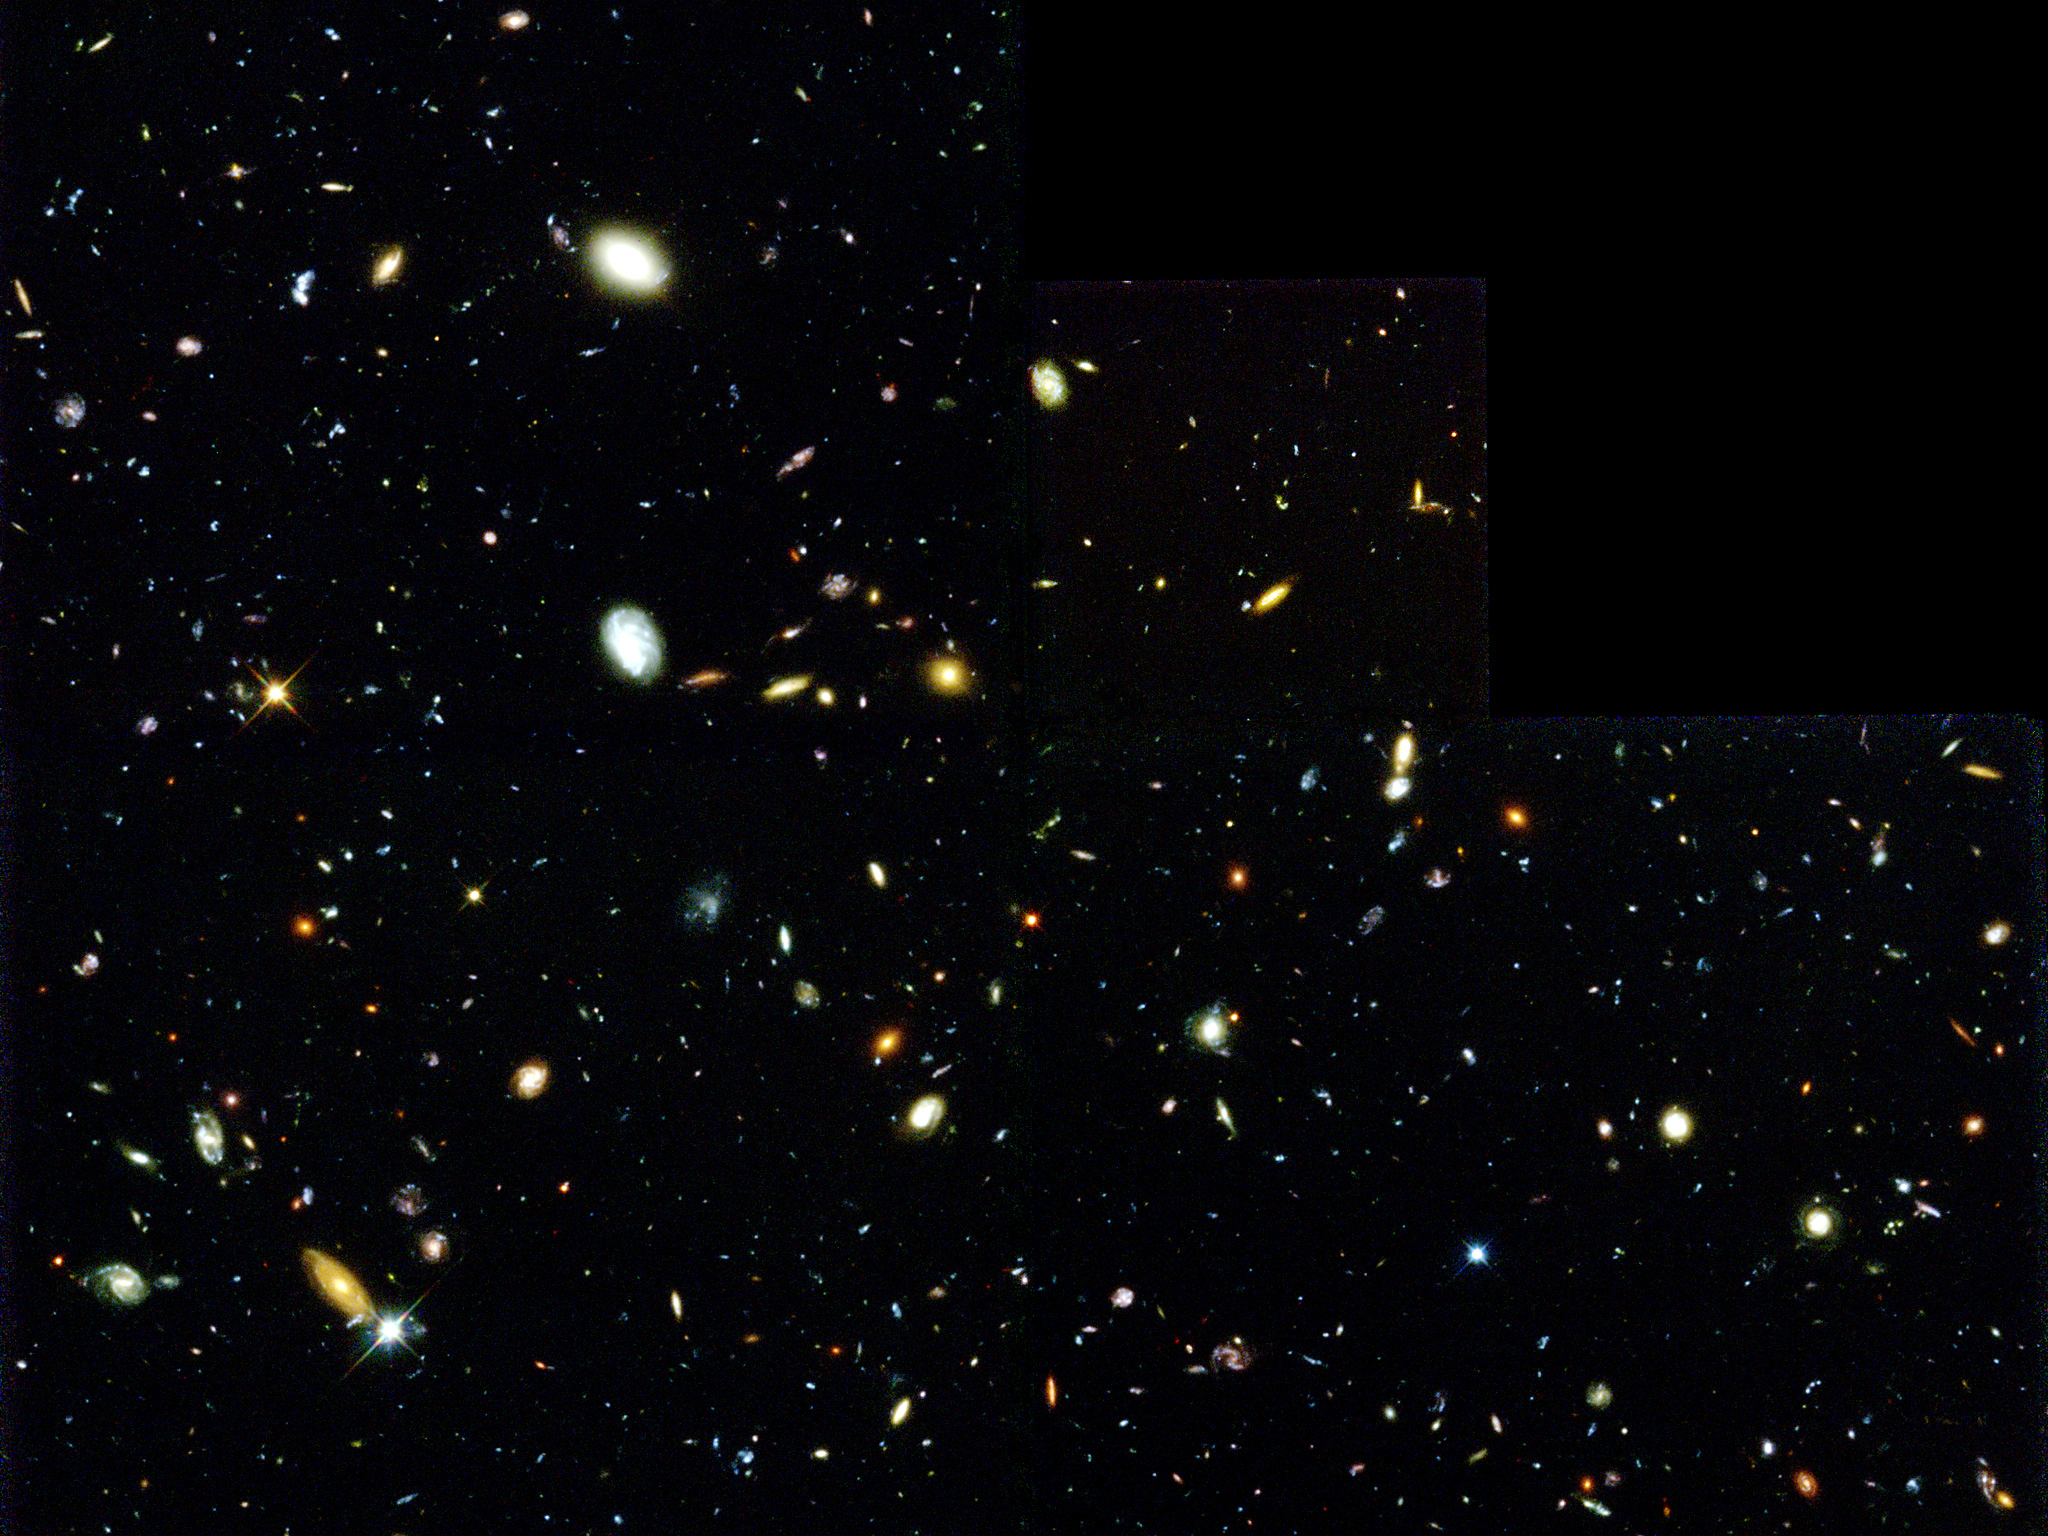
\includegraphics[width=0.9\columnwidth]{Figures/hubble_deep_field.jpeg}
	\caption{The Hubble Deep Field as captured by the Wide Field and Planetary Camera 2 onboard the \textit{Hubble Space Telescope} in 1995.}
	\label{fig:hubble_deep_field}
\end{figure}

\section{Galaxy Formation and Evolution}

To answer our questions on the evolution of galaxies, we must first make some inferences about the {\color{red}[...]} of the Universe. Our understanding of the cosmic history of galaxies is dependent on our choice of cosmology, which is widely accepted to be in the form of the $\Lambda$-CDM model (\citealt{Peebles_1980}). In the $\Lambda$-CDM model, Cold Dark Matter, matter of unknown origin, dominates over ordinary baryonic matter; and with dark energy, constitute a combined $\sim 95\%$ of the total cosmic energy budget ({\color{red}REFERENCE}). The presence of dark matter is only evident in its gravitational interactions with other matter, but its origin is unknown as it does not interact with nor emit any electromagnetic radiation. The dark energy in the Universe is parameterized in the form of the cosmological constant, $\Lambda$, which is required to explain the accelerating expansion of the Universe. In this model, galaxy formation is seeded by small quantum fluctuations in the density of the early Universe, which grow with inflation to form small overdensities that later become the sites of dark matter halos by gravitationally attracting nearby dark matter. The first galaxies formed from these originally minute overdensities in density, which later merge due to an increase in collisions in a smaller Universe, to form ever larger galaxies. This model of galaxy formation is called a 'hierarchical' model, where galaxies in the early Universe are expected to be smaller and formed their mass more quickly than massive galaxies at later times that formed much of their stellar mass from previous mergers. As we shall show in Chapter \ref{chapter:Radio_Identifications}, this model of evolution may not explain the stellar build up of all galaxies.

\subsection{Classification of Galaxies}

The first step in understanding galaxy evolution by observing how galaxies have changed as we look back in time, is to classify galaxies according to their observable properties. Generally, galaxies can be classified into two broad groups based on their morphology: spirals and ellipticals. This dichotomy prompted the first classification scheme by Edwin Hubble (Figure \ref{fig:hubble_tuning_fork}; \citealt{Hubble_1936}), the \textit{Tuning Fork}, which shows ellitpical galaxies along the "handle", becoming more oblate towards the spiral galaxies. The spiral galaxies themselves are split into two categories forming the two "prongs", depending on the presence of a bar at the centre. At the join of the two, is where we might locate \textit{lenticular galaxies}, that are recognized by their large disks, like spirals, but without the presence of arms. In the rest of this Thesis we shall predominantly be referring to elliptical galaxies at \textit{early-type galaxies} (ETGs) and spiral-like galaxies as \textit{late-type galaxies} (LTGs), as is convention. Despite their names, the two do not represent a former and latter evolutionary stage of a typical galaxy, and is rather a misnomer. A minority of galaxies do not conform to this dichotomous image and are typically grouped together as \textit{irregular galaxies}.

\begin{figure}
    \centering
	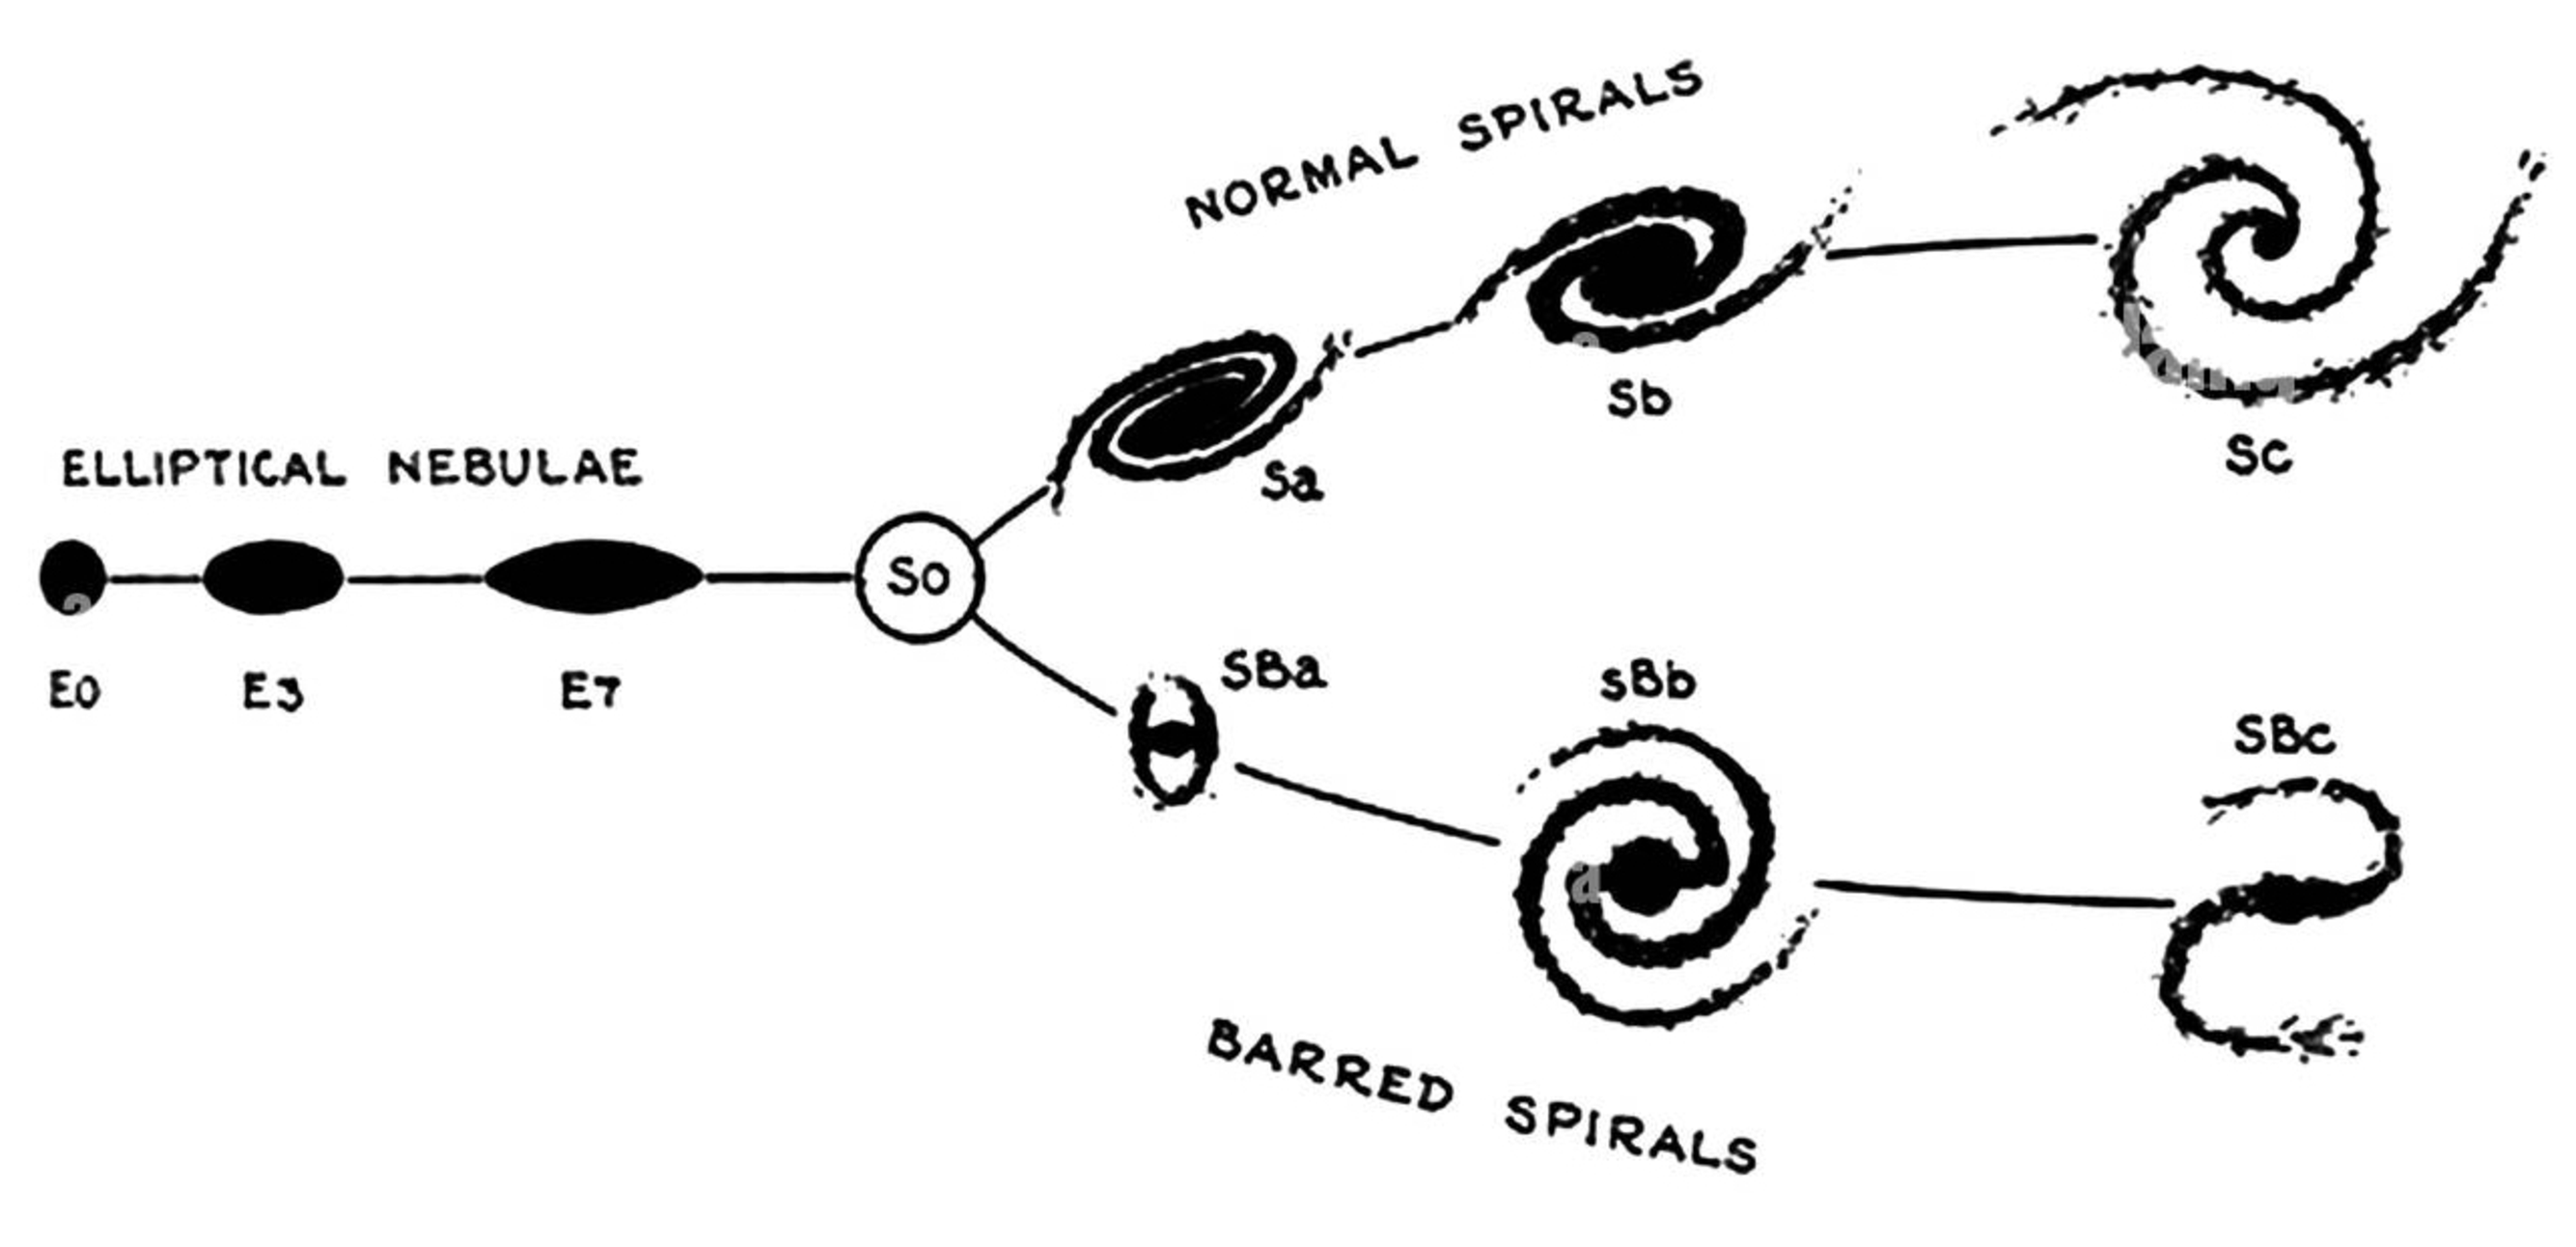
\includegraphics[width=0.9\columnwidth]{Figures/hubble_tuning_fork}
	\caption{The \textit{Hubble Tuning Fork}, or the \textit{Sequence of Nebular Types} as named in \citealt{Hubble_1936}, showing spiral galaxies along the prongs of the tuning fork and elliptical galaxies along the handle. The two prongs separate those spiral galaxies with barred central bulges from those that do not. Lenticular galaxies can be found at the join of the handle to the prongs. From left to right, the elliptical galaxies become more oblate and the spiral galaxies have spiral arms that become less tightly wound around the central bulge.}
	\label{fig:hubble_tuning_fork}
\end{figure}

Beyond their shape, the two broad groups, ETGs and LTGs, have a number of physical characteristics that are often shared among their population. The stellar content of ETGs is dominated by older, cooler stellar populations that typically have red colours. These galaxies are largely devoid of gas and are expected to have very little active star formation. In contrast, LTGs have spiral arms that contain active regions of star formation, and thus have younger, hotter, more massive stars that appear more blue in colour.

The fractional share of galaxies between the two categories has evolved with time ({\color{red}REFERENCE}) which points to {\color{red}[... Look at Matt's notes ...]}

\subsection{The Main Sequence of Star Formation}